\documentclass[a4paper]{article}
\usepackage{a4wide}
\usepackage{amsmath}
\usepackage{amsfonts}
  \DeclareMathOperator*{\argmax}{arg\,max}
  \newcommand{\ex}[1]{{\mathbb E}\left[ #1 \right]}
  \newcommand\norm[1]{\left\lVert#1\right\rVert}
\usepackage{booktabs}
\usepackage{csquotes}
\usepackage{upquote}
\usepackage{float}
\usepackage{graphicx}
\usepackage{enumerate}
\usepackage{subcaption}
\usepackage{xcolor}


\title{Pattern and Speech Recognition WS2015-16 \\ Exercise 6}
\author{Atanas Poibrenski(2554135), Marimuthu Kalimuthu(2557695), Furkat Kochkarov(2557017)}

\begin{document}

\maketitle 
\begin{center}
	\textbf{EM algorithm for Gaussian Mixture Models}
\end{center}

\section*{Exercise 1}
\begin{enumerate}
	\item[ \textbf{1} ] Done.
	\item[ \textbf{2} ] See ``data\_preparation.m"

	\begin{figure}[H]
		\begin{center}
			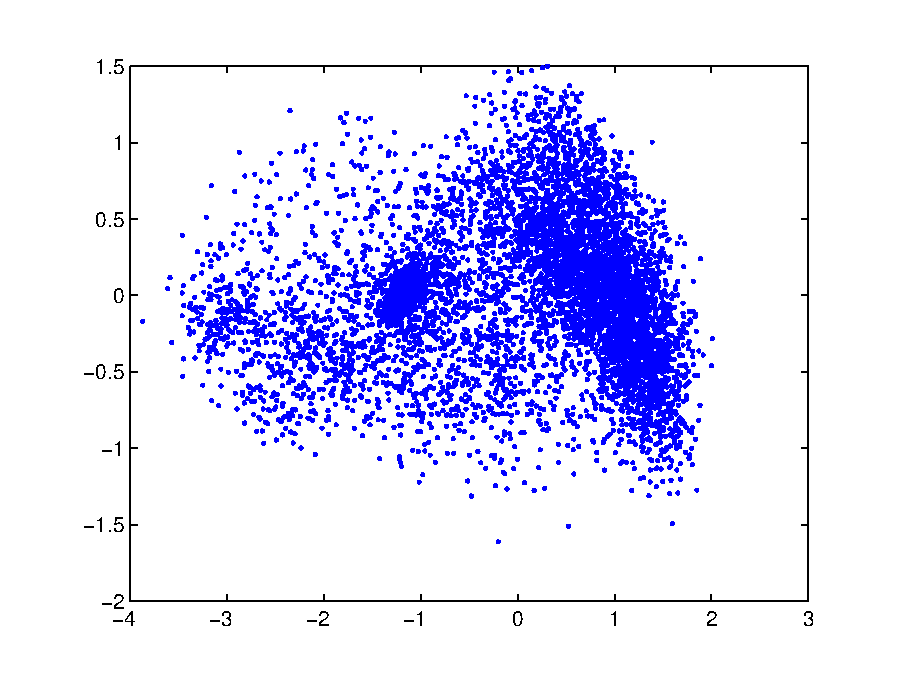
\includegraphics[width=0.9\textwidth]{data_plot.eps}
			\caption{Transformed data distribution}\label{fig:transdata}
		\end{center}
	\end{figure}

	\item[ \textbf{3} ] See ``GMM.m"
	\item[ \textbf{4} ] See ``GMM.m"
	\item[ \textbf{5} ] See ``GMM.m"
	\item[ \textbf{6} ] See ``GMM.m". We calculated the covariance matrix of the transformed data in (2) and from that we can observe that it is indeed a diagonal matrix.
	\item[ \textbf{7} ] In each iteration, after updating the \textit{mean}, we compare it with the \textit{mean} of previous iteration. If the difference between them is less than the threshold of 0.0001 ($10^{-4}$), we stop further iterations.
	\item[ \textbf{8} ] Plots for K={2,4,10} and multiple runs.
	
		\begin{figure}[H]
			\begin{center}
				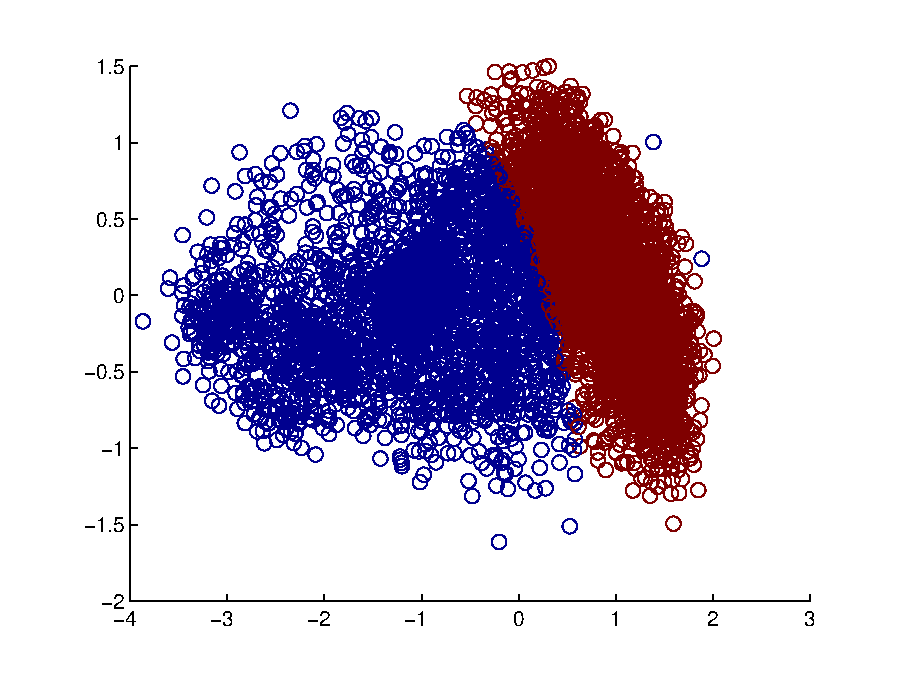
\includegraphics[width=0.8\textwidth]{GMM_K2.eps}
				\caption{GMM clusters for K=2}\label{fig:gmm_k2}
			\end{center}
		\end{figure}

		\begin{figure}[H]
			\begin{center}
				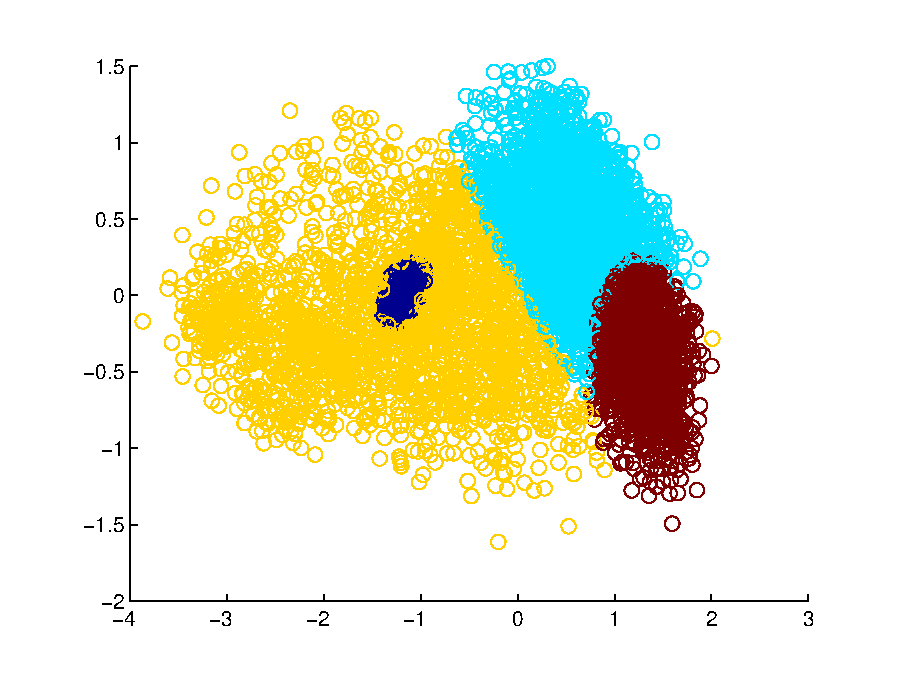
\includegraphics[width=0.8\textwidth]{GMM_K4.eps}
				\caption{GMM clusters(run-1) for K=4}\label{fig:gmm_k4}
			\end{center}
		\end{figure}

		\begin{figure}[H]
			\begin{center}
				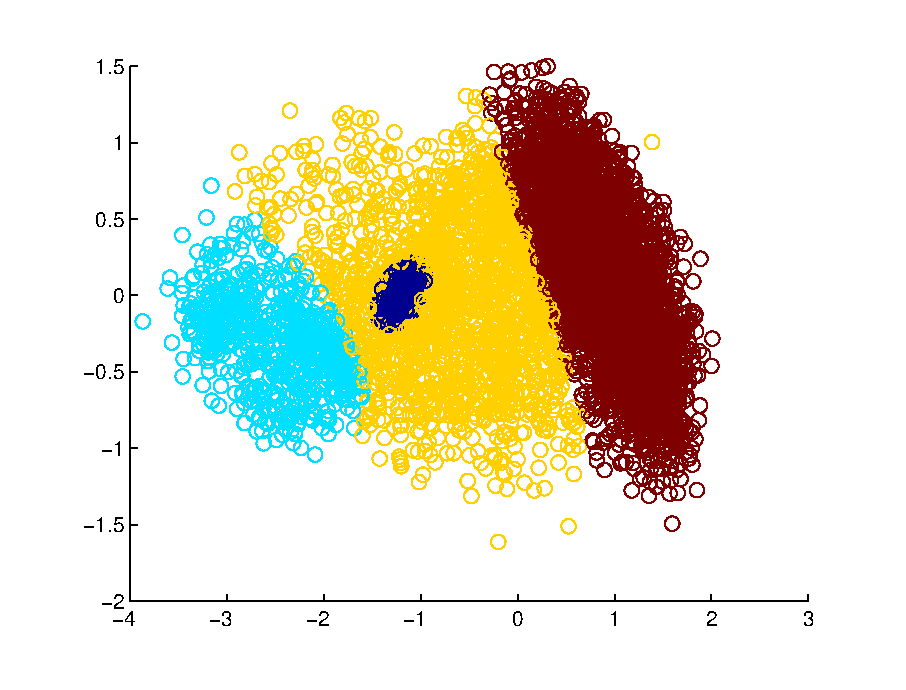
\includegraphics[width=0.8\textwidth]{GMM_K4_1.eps}
				\caption{GMM clusters(run-2) for K=4}\label{fig:gmm_k4_1}
			\end{center}
		\end{figure}

		\begin{figure}[H]
			\begin{center}
				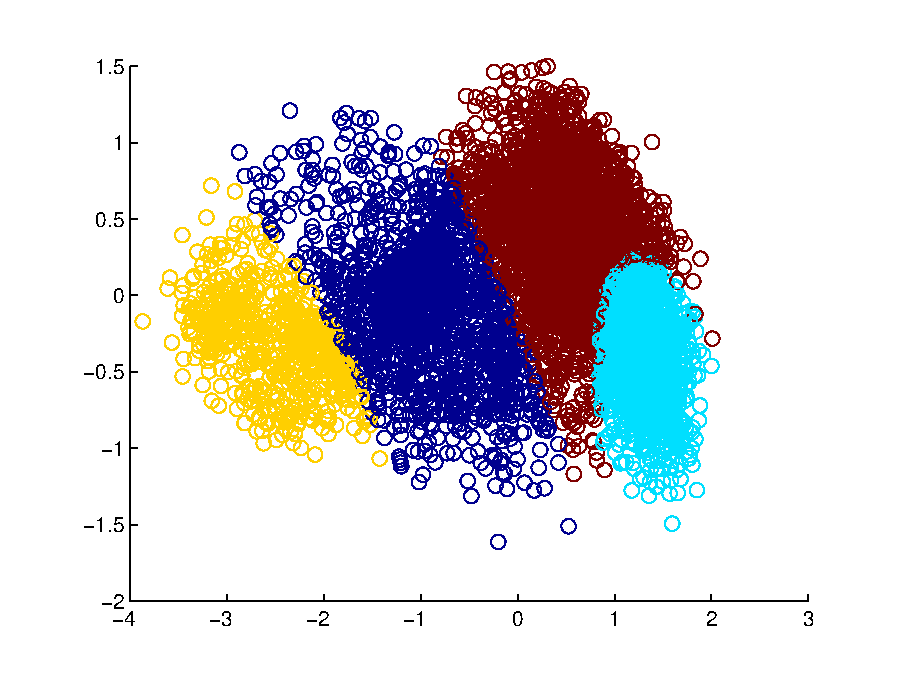
\includegraphics[width=0.8\textwidth]{GMM_K4_2.eps}
				\caption{GMM clusters(run-3) for K=4}\label{fig:gmm_k4_2}
			\end{center}
		\end{figure}		


		\begin{figure}[H]
			\begin{center}
				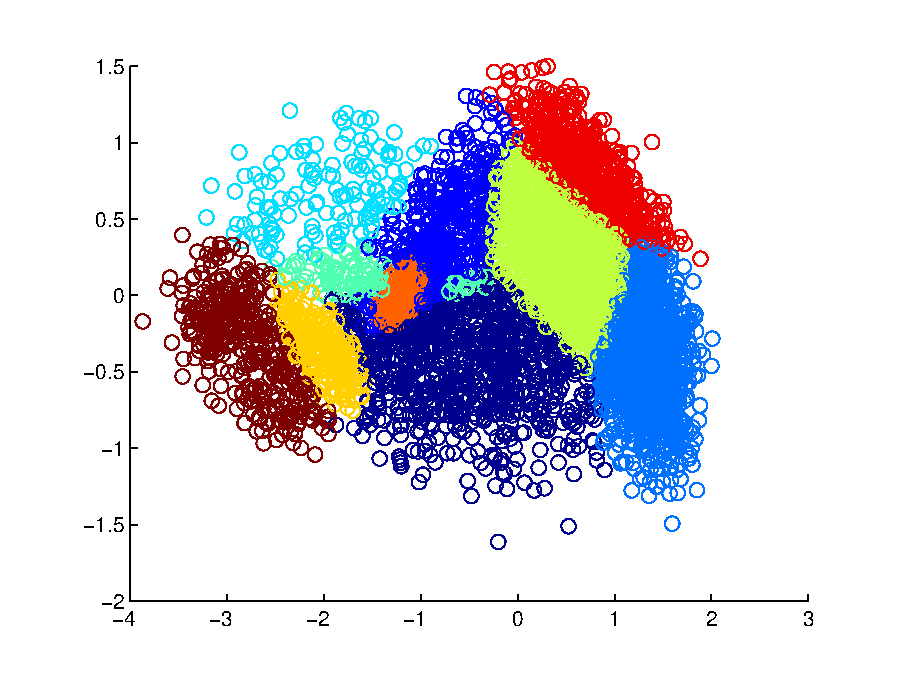
\includegraphics[width=0.8\textwidth]{GMM_K10.eps}
				\caption{GMM clusters(run-1) for K=10}\label{fig:gmm_k10}
			\end{center}
		\end{figure}
		
		\begin{figure}[H]
			\begin{center}
				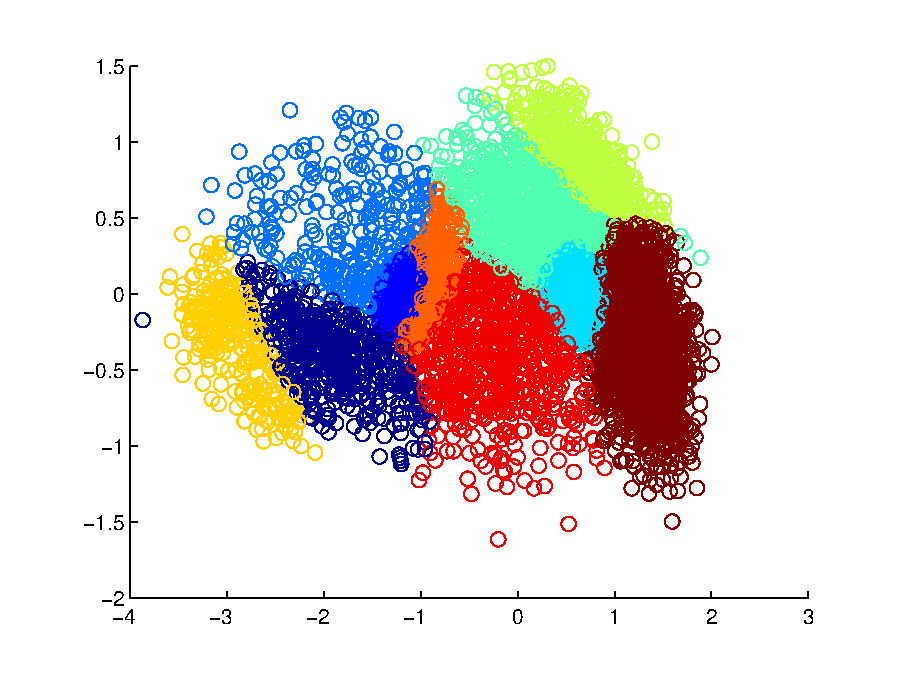
\includegraphics[width=0.8\textwidth]{GMM_K10_1.eps}
				\caption{GMM clusters(run-2) for K=10}\label{fig:gmm_k10_1}
			\end{center}
		\end{figure}
		
		\begin{figure}[H]
			\begin{center}
				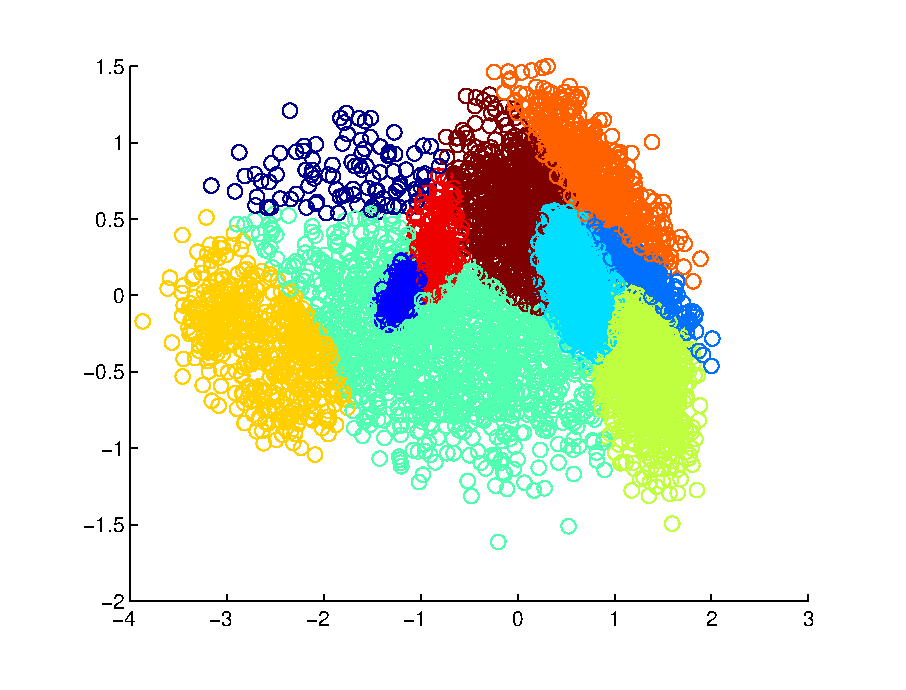
\includegraphics[width=0.8\textwidth]{GMM_K10_2.eps}
				\caption{GMM clusters(run-3) for K=10}\label{fig:gmm_k10_2}
			\end{center}
		\end{figure}


	\item[ \textbf{9} ] GMM is a soft-clustering which assigns a probability for each data point to which potential cluster it may belong to. The boundaries between the clusters is not linear. 
	\item[ \textbf{10} ] Plots for K-Means
		\begin{figure}[H]
			\begin{center}
				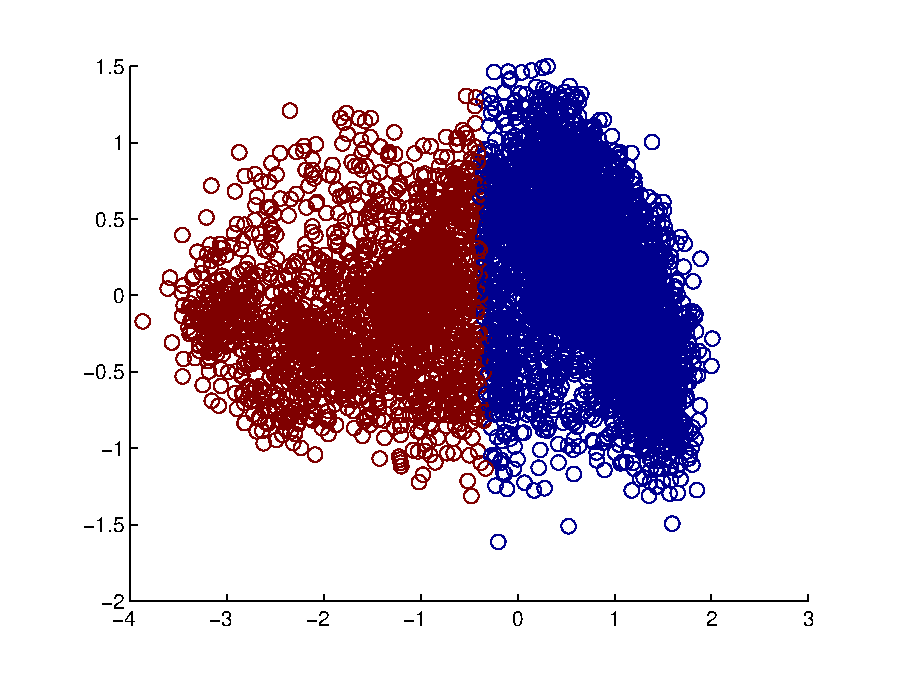
\includegraphics[width=0.8\textwidth]{KMEANS_K2.eps}
				\caption{K-Means clusters for K=2}\label{fig:kmeans_k2}
			\end{center}
		\end{figure}

		\begin{figure}[H]
			\begin{center}
				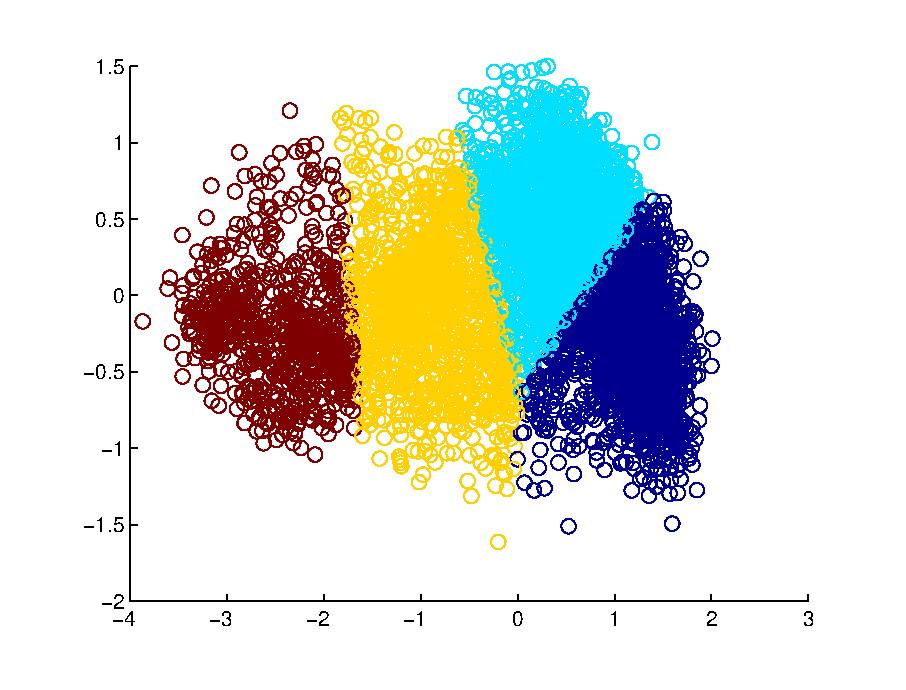
\includegraphics[width=0.8\textwidth]{KMEANS_K4.eps}
				\caption{K-Means clusters for K=4}\label{fig:kmeans_k4}
			\end{center}
		\end{figure}
			
		\begin{figure}[H]
			\begin{center}
				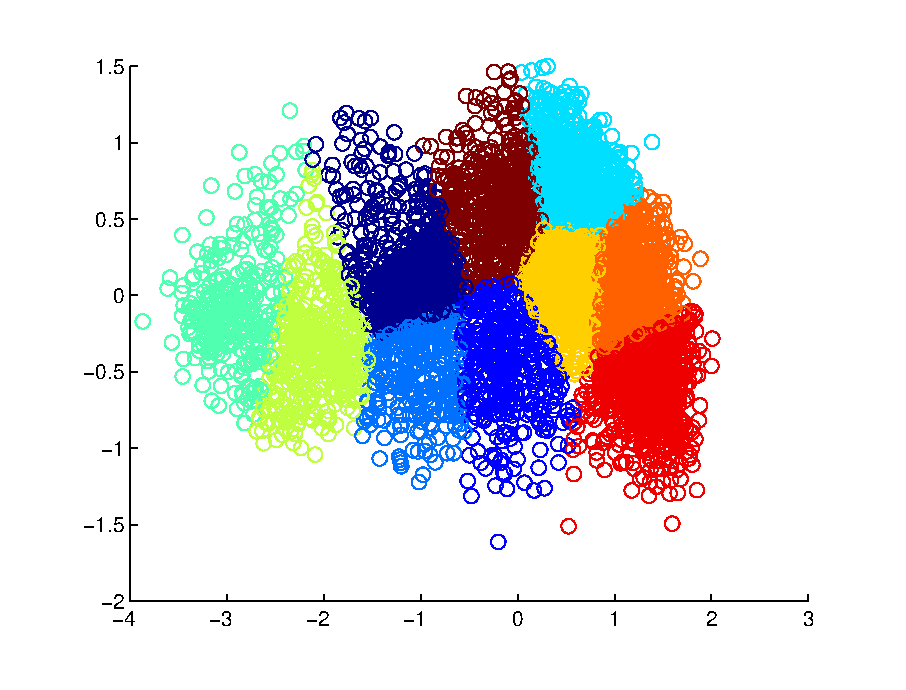
\includegraphics[width=0.8\textwidth]{KMEANS_K10.eps}
				\caption{K-Means clusters for K=10}\label{fig:kmeans_k10}
			\end{center}
		\end{figure}
		
		\textbf{Differences}: 
		\begin{itemize}
			\item K-means clusters the data points with linear decision boundary like voronoi diagram whereas GMM provides soft clustering with non-linear decision boundary. 
			\item In K-means, which is a hard clustering, the data points either belong to one cluster or the other. But GMM gives a probability for the data points being in a particular cluster.(In our case, we finally assign the data points to the cluster with highest posterior probability.)
			\item From the above figures, we can see that GMM allows clustering inside clustering whereas this is not possible with K-means.
		\end{itemize}
\end{enumerate}

\section*{Exercise-2; BONUS}
The center of mass in each cluster of GMM is relatively the same as the center of mass of each cluster in Kmeans. \newline
The plots are given below.
		\begin{figure}[H]
			\begin{center}
				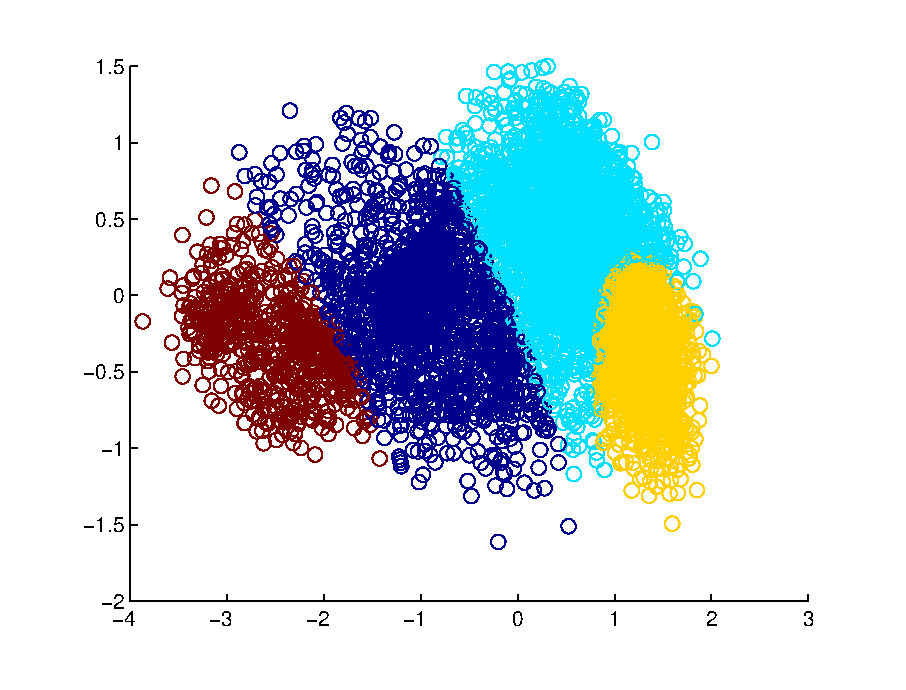
\includegraphics[width=0.8\textwidth]{GMM_KMEANS_K4.eps}
				\caption{GMM2 clusters for K=4}\label{fig:gmm_kmeans_k4}
			\end{center}
		\end{figure}
		
		\begin{figure}[H]
			\begin{center}
				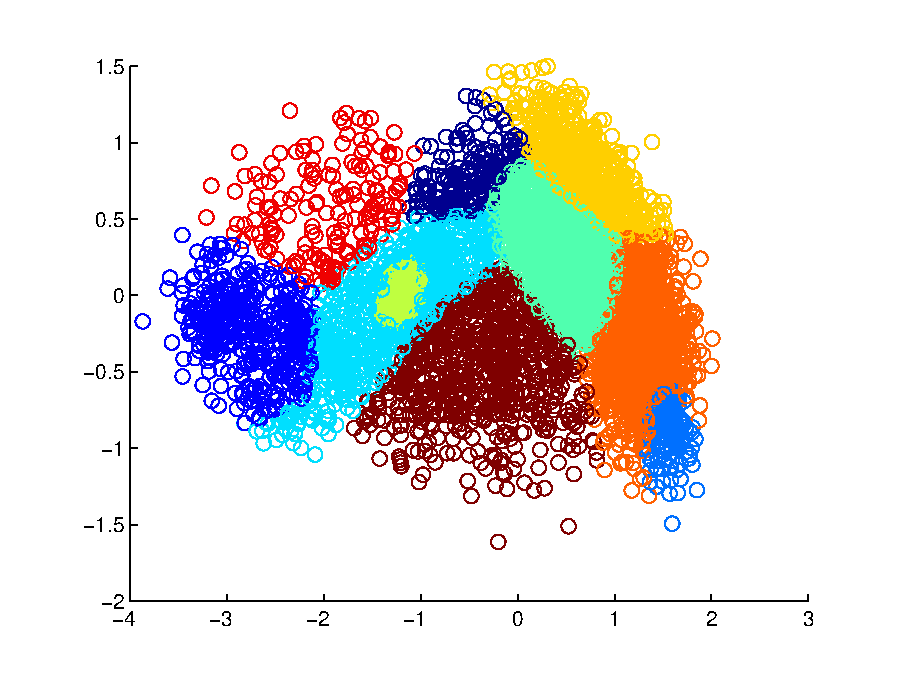
\includegraphics[width=0.8\textwidth]{GMM_KMEANS_K10.eps}
				\caption{GMM2 clusters for K=10}\label{fig:gmm_kmeans_k10}
			\end{center}
		\end{figure}

\end{document}
